\section{High level design description}
\begin{figure}[!ht]
 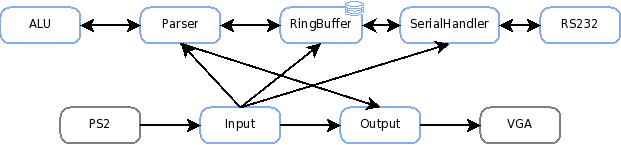
\includegraphics[scale=0.55]{pics/Modules.png}
 % Modules.png: 501x145 pixel, 72dpi, 17.67x5.12 cm, bb=0 0 501 145
 \label{fig:Modules}
\end{figure}

%%%%%%%%TODO Beschreibung der Submodule
% HIER REIN
\subsection{Logical Interfaces}
Die schon gezeigten Module besitzen folgende I/Os:
\begin{figure}[!ht]
 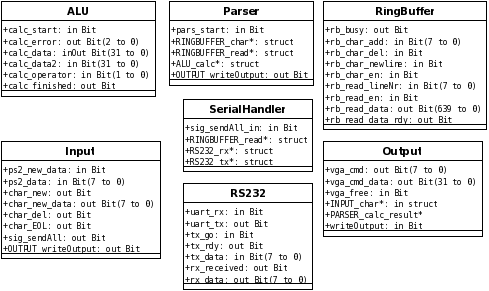
\includegraphics[scale=0.7]{pics/Klassen.png}
 % Modules.png: 501x145 pixel, 72dpi, 17.67x5.12 cm, bb=0 0 501 145
 \label{fig:Klassen}
\end{figure}


\subsection{Behavioural Interface}
\subsubsection{Output on the screen}
Der Bildschirm kann 80 Zeichen in einer Zeile darstellen und unsere Rechnung kann 70 Zeichen lang sein. Mit einem '=' Zeichen würden uns 9 Zeichen für das Ergebnis bleiben. Unser Ergebnis ist jedoch 32 Bit lang und liegt zwischen [2147483648,-2147483647].\\
Deswegen und auch wegen der Übersicht schreiben wir das Ergebnis in die nächste Zeile.\\
Der Bildschirmhintergrund ist schwarz mit weißer Schrift. Die Rechnung beginnt in der ersten Zeile. Sollten keine Zeilen mehr frei sein rutschen alle Rechnungen nach oben und die Älteste wird gelöscht.
\subsubsection{Output on the RS232}
Wird der Button am Developer board, oder eine bestimmte Taste am PC, gedrückt, wird der gesamte Verlauf der letzten 50 Rechnungen mit den Ergebnissen an den PC geschickt.
\subsubsection{What about overflows?}
Overflows werden von unserem ALU Modul abgefangen. Tritt ein Overflow auf wird die Berechnung beendet und eine Fehlernachricht in die History gespeichert.
\subsubsection{Allowed keyboard input}
%%%%%%%%%%%%%%%%%%%%%%%%%%%%%%%%%%%%%%%%%%%
%%%Input from detailed design description
%%%%%%%%%%%%%%%%%%%%%%%%%%%%%%%%%%%%%%%%%%%
Das Programm reagiert nur auf gedrückte und nicht auf losgelassene Tasten. Weiters verwenden wir die Scankeys der 
Zahlen und Operatoren vom NumPad und Enter, Leertaste und Backspace von der Haupttastatur.
\begin{center}
\begin{tabular}{|l|l|l|}
\hline ASCII & Scankey (Set2) & ASCII (hex)\\
\hline 0 & 0x70 & 30\\
1 & 0x69 & 31\\
2 & 0x72 & 32\\
3 & 0x7a & 33\\
4 & 0x6b & 34\\
5 & 0x73 & 35\\
6 & 0x74 & 36\\
7 & 0x6c & 37\\
8 & 0x75 & 38\\
9 & 0x7d & 39\\
+ & 0x79 & 2B\\
- & 0x7b & 2D\\
/ & 0xe0 0x4a & 2F\\
$*$ & 0x7c & 2A\\
Backspace & 0x66 & 08\\
Enter & 0x5a & 0A\\
Space & 0x29 & 20\\
\hline

\end{tabular}
\end{center}
\subsubsection{Erroneous inputs}
Alle Tasten die nicht spezifiziert sind werden verworfen. Bei fehlerhaften Eingaben wird der Fehler vom Parser und der ALU abgefangen, die Zwischenergebnisse verworfen, die entsprechende Fehlernachricht am Bildschirm ausgegeben und in der History gespeichert.
\subsubsection{Error messages}
Wir unterscheiden zwischen drei Fehlernachrichten:
\begin{description}
 \item[Overflow] Wenn bei irgendeiner Berechnung ein Overflow Fehler auftritt. 
 \item[Division durch Null] Sollte bei Irgendeiner Division im Zähler null stehen wird diese Nachricht ausgegeben.
 \item[falscher Syntax]Zu falscher Syntax zählt ein Operand am Ende, zwei Operanden hintereinander oder eine Punktrechnung am Anfang.
\end{description}


\subsection{Physical Interfaces}
Die Physikalischen Interfaces der gesamten angeschlossenen Hardware lässt sich
in nachfolgender Pintabelle ablesen.
\begin{table}[!ht]
 \begin{center}
  \begin{tabular}{|l|l|l|l|}
   \hline Signal & Pin &Direction &Logic Level\\
   sys\_clk & N3 & in & LVTTL\\
   sys\_res\_n & AF17 & in & LVTT\\
   btn\_a & A3 & in & LVTTL\\
   uart\_cts & D20 & out & LVTTL\\
   uart\_rts & D21 & in & LVTTL\\
   uart\_txd & D22 & out & LVTTL\\
   uart\_rxd & D23 & in & LVTTL\\
   ps2\_data & E21 & bidirec & LVTTL\\
   ps2\_clk & Y26 & bidirect & LVTTL\\
   vga\_r0 & E22 & out & LVTTL\\
   vga\_r1 & T4 & out & LVTTL\\
   vga\_r2 & T7 & out & LVTTL\\
   vga\_g0 & E23 & out & LVTTL\\
   vga\_g1 & T5 & out & LVTTL\\
   vga\_g2 & T24 & out & LVTTL\\
   vga\_b0 & E24 & out & LVTTL\\
   vga\_b1 & T6 & out & LVTTL\\
   vga\_hsync\_n & F1 & out & LVTTL\\
   vga\_vsync\_n & F2 & out & LVTTL\\
   \hline
  \end{tabular}
 \end{center}
\end{table}


\subsection{Reset and Clock}
Der Reset wurde low active gewaehlt.

Der VGA Controller wird über eine PLL auf 25.175 MHz getaktet. 
Alle weiteren Controller benützen die externe Clockfrequenz
des Developer Boards von 33.33 MHz.

